% ============================================================
% Sterman (2008) climate stabilization task -- original figures
% extracted from the Science article as vector PDF crops.
%
% Requires the three PDF files in the figures/ folder:
%   sterman_scenario.pdf, sterman_task.pdf, sterman_response.pdf
% (\graphicspath{{figures/}} is already set in main.tex)
% ============================================================

\begin{figure}[htbp]
    \centering
    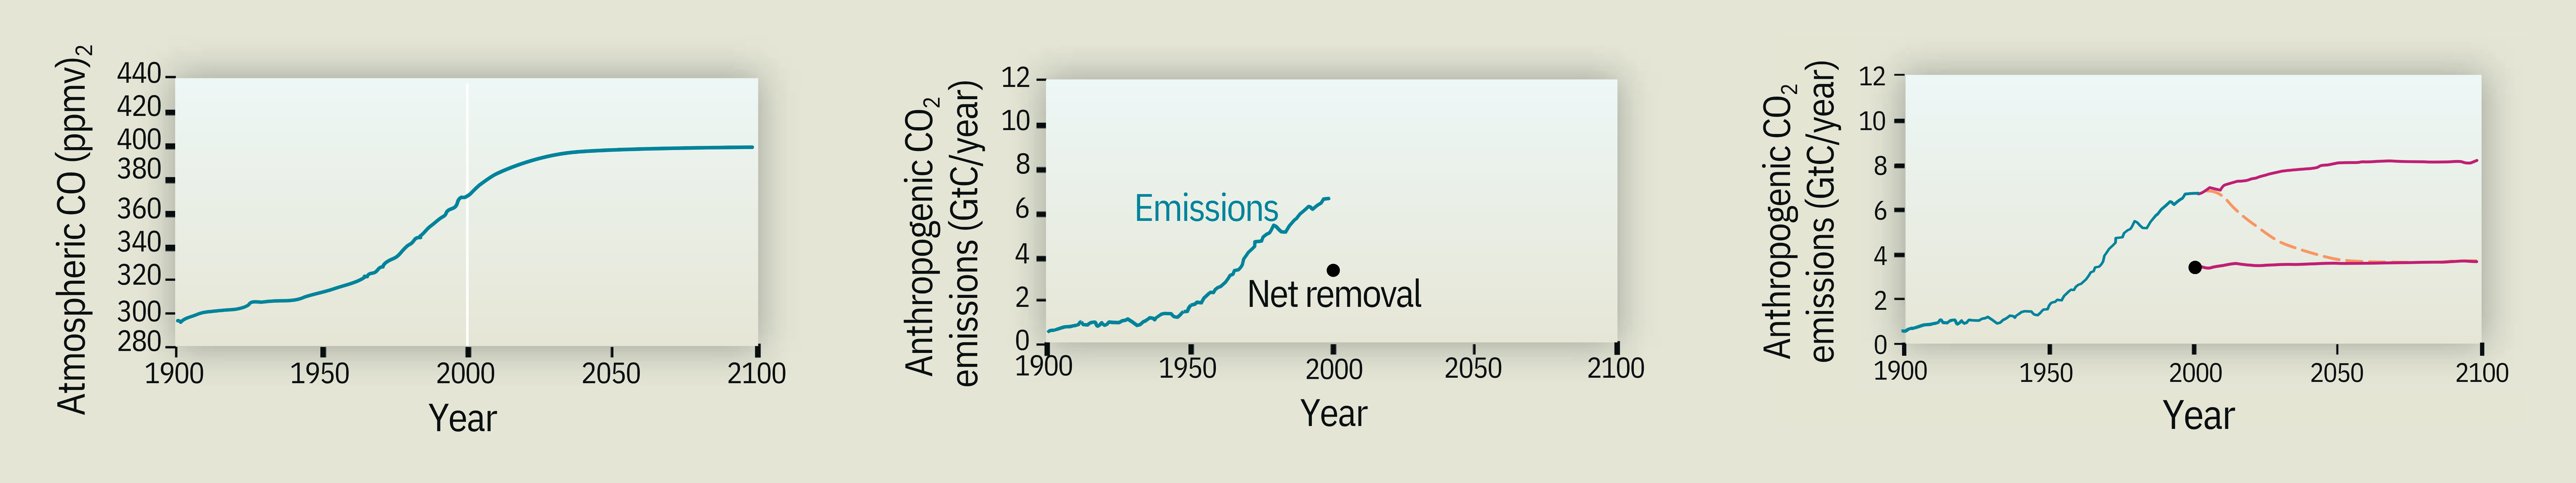
\includegraphics[width=\textwidth]{sterman_panel.png}
    \caption[The climate stabilization task]{The climate stabilization
    task. (a)~The scenario presented to participants: atmospheric
    CO\textsubscript{2} concentration rises gradually to 400~ppmv and
    stabilizes by 2100. (b)~The stock--flow information provided:
    anthropogenic CO\textsubscript{2} emissions from 1900 to 2000 (the
    inflow) and current net removal by oceans and biomass (the
    outflow), with emissions roughly double net removal. (c)~A typical
    response: participants erroneously sketch future emissions that
    match the shape of the CO\textsubscript{2} trajectory
    (pattern-matching heuristic), while mass balance requires emissions
    to fall until they equal net removal (dashed line). Reprinted from
    \citet{sterman2008}.}
    \label{fig:sterman-panel}
\end{figure}